Cette section décrit deux leviers pour améliorer la sécurisation et la résilience des chaînes d'approvisionnement : la maîtrise technologique et le recyclage.\smallbreak
Au-delà d'être une première étape pour disposer de technologie bas-carbone, la maîtrise technologique doit s'entendre comme la maîtrise des technologies. Disposer d'un éventail de technologies bas-carbone permet de substituer certains métaux par des éléments plus accessibles, ou d'en réduire la quantité nécessaire à service identique. La maîtrise technologique peut aussi avoir un rôle dans l'amélioration de la durée de vie des technologies bas-carbone et donc dans le besoin en métaux critiques. En résumé, une maîtrise technologique plus fine permet aux Etats de donner plus de flexibilité à leur besoin en métaux et donc de réduire le risque géopolitique.\smallbreak
Le recyclage permet d'offrir une source d'approvisionnement dite "secondaire". L'enjeu autour du recyclage est de collecter la ressource et de développer un modèle économique pour les filières du recyclage.
\subsubsection{Technologie}
\begin{figure}[!b]
    \centering
    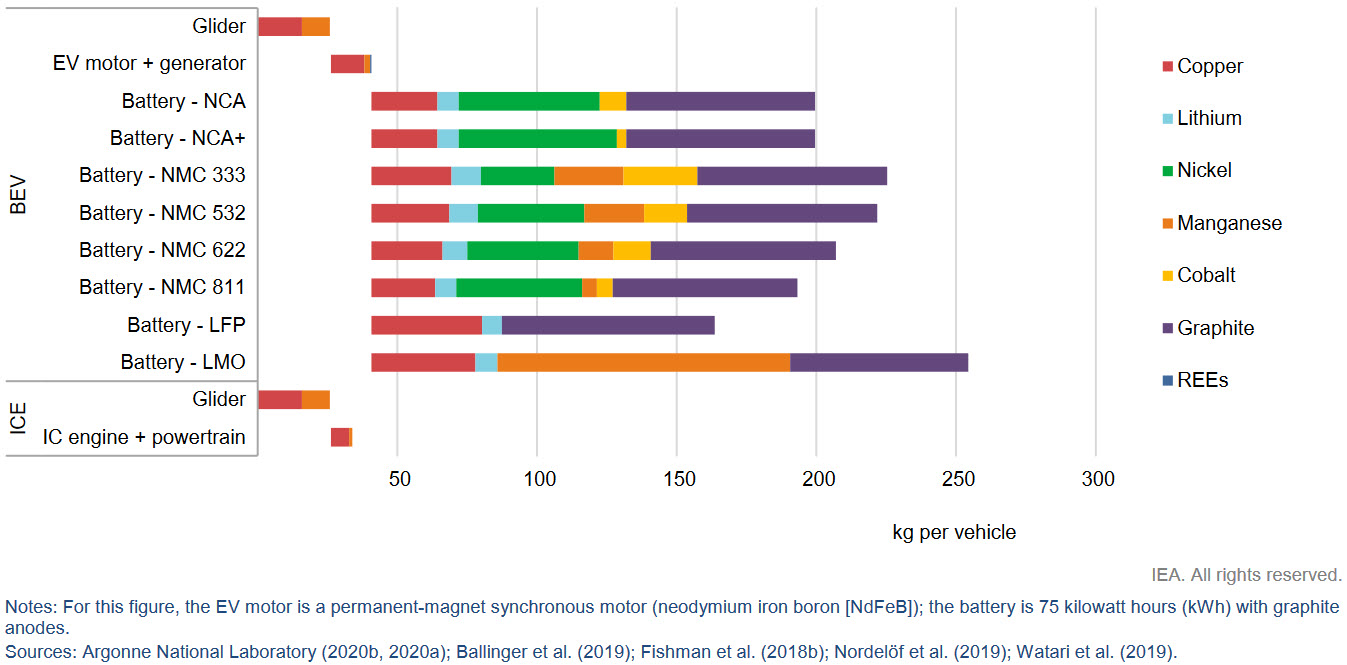
\includegraphics[width=0.8\textwidth]{Images/supply_chain/metals_by_battery.jpg}
    \caption{Utilisation de métal dans une voiture thermique (ICE) ou électrique (BEV) avec plusieurs batteries possible (\cite{iea_role_2021})}
    \label{fig:batteries}
\end{figure}
~\\
\textbf{Eolien}
\smallbreak
La maîtrise technologique dans l'éolien se joue surtout dans l'aptitude à construire des éoliennes de grande capacité. En plus de permettre une réduction de la quantité de métal par MW, ces éoliennes ont un facteur de charge plus élevé, produisant plus d'électricité pour la même quantité de matériaux. L'utilisation de générateur synchrone à excitation électrique à la place de générateur synchrone à aimant permanent permet de réduire de plus de 70\% la quantité de terres rares requise par MW (\cite{iea_role_2021}).
\bigbreak
\textbf{Photovoltaïque}
\smallbreak
Différentes technologies peuvent affecter les composants requis pour les semi-conducteurs, mais avec peu de conséquences sur les métaux critiques. En revanche, il est à noter que les installations photovoltaïques diffuses nécessitent en moyenne 40\% de cuivre en plus à cause d'un plus grand besoin en électronique de puissance et d'une moins bonne efficacité (\cite{iea_role_2021}).
\bigbreak
\textbf{Réseaux électriques}\smallbreak
La substition du cuivre par de l'aluminum est envisageable pour les lignes aériennes, car bien qu'étant moins conducteur, l'aluminum est plus léger. L'adoption et l'intégration du courant continu dans le réseau électrique pourraient permettre de diminuer de 15\% la demande mondiale de cuivre et d'aluminium pour les réseaux électriques. En théorie, deux câbles en courant continu peuvent transporter jusqu'à 3.5 fois plus d'électricité que trois câbles de même diamètre en courant triphasé (\cite{iea_role_2021}).
\bigbreak
\textbf{Batteries}
\smallbreak
Actuellement, plusieurs compositions chimiques sont possibles pour les cathodes des batteries lithium-ion : lithium cobalt oxide (LCO), lithium manganese oxide (LMO), lithium fer phosphate (LFP), lithium nickel cobalt aluminium oxide (NCA) et lithium manganese cobalt oxide (NMC). Plusieurs proportions sont possibles parmi les compositions chimiques proposées. Cet éventail de batteries permet des besoins en métaux variables (figure \ref{fig:batteries}). Les caractéristiques à apprécier pour les batteries des véhicules électriques sont la densité énergétique, la stabilité thermique et la durée de vie. Durant ces dernières années, une hausse des prix du cobalt ont incité à développer des batteries qui substituent le cobalt par du nickel. Ainsi, la batterie NCA a transitionné vers la batterie NCA + (voir figure \ref{fig:batteries}).
\smallbreak
Une percée dans la performance des batteries est possible grâce à l'avènement des batteries lithium solide (ASSBs). Ce type de batterie n'a pas d'électrolyte liquide. Cette technologie permettrait de faire passer la densité énergétique de 300 Wh/kg à 480 Wh/kg réduisant ainsi le besoin de métaux.
\begin{figure}[!t]
    \centering
    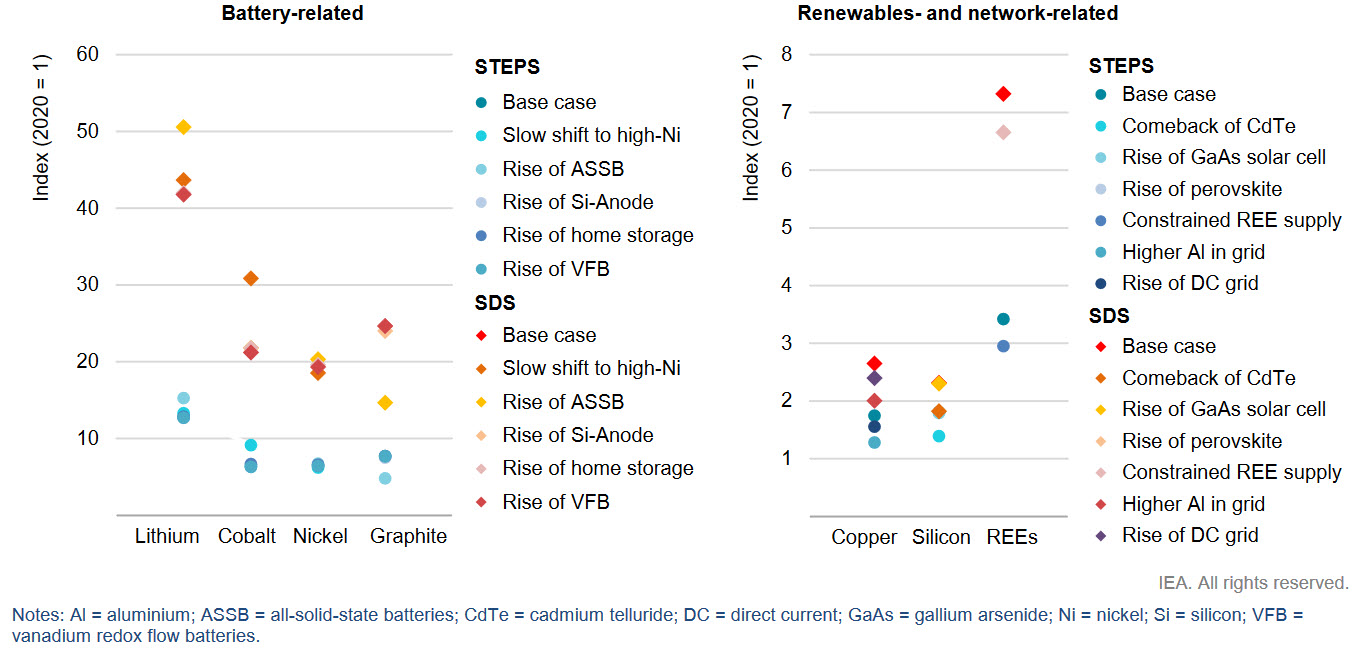
\includegraphics[width=0.8\textwidth]{Images/supply_chain/levier_techno.jpg}
    \caption{Demande mondiale en minéraux pour les technologies bas-carbone en 2040 relativement à 2020 selon plusieurs scénarios et tendances (\cite{iea_role_2021})}
    \caption*{Note : 'Comeback of CdTe','Rise of GaAs solar cell' et 'Rise of perovskite' sont des changements de tendances dans les semi-conducteurs du photovoltaïque}
    \label{fig:techno_levier}
\end{figure}

\begin{center}
    \boxput*(0,1){
        \colorbox{white}{Propriété intellectuelle}
    }{
    \setlength{\fboxsep}{15pt}
    \fbox{\begin{minipage}{14cm} 
    \begin{center}
    \textit{Nombre de brevets déposés chaque année}
        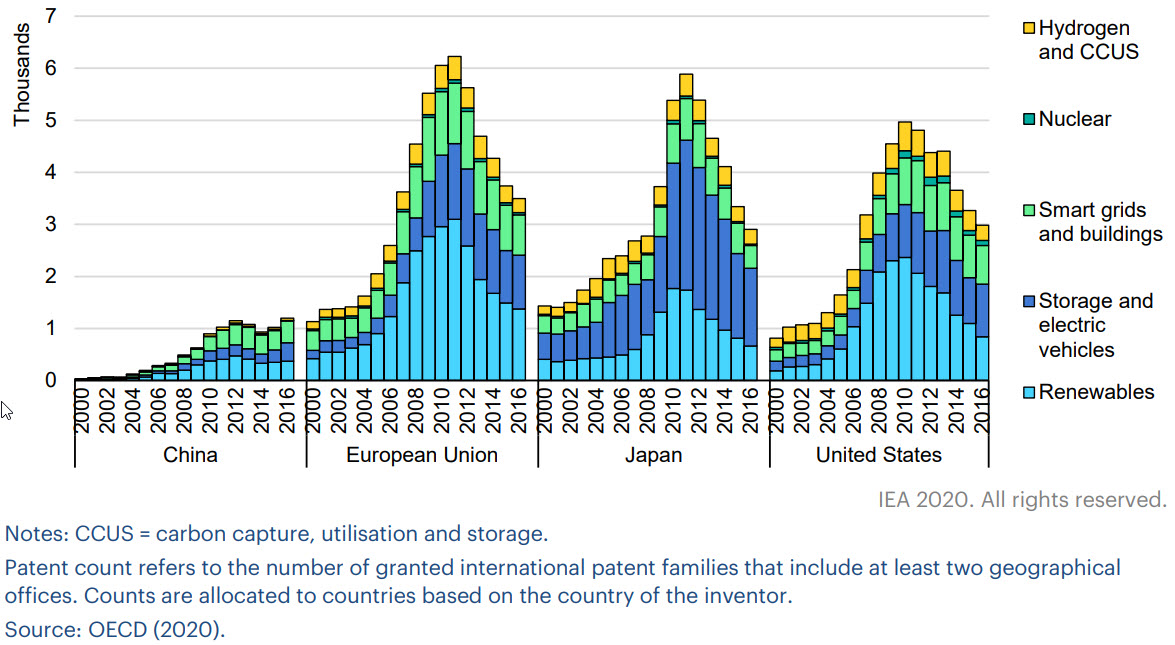
\includegraphics[width=10cm]{Images/supply_chain/brevet.jpg}
    \end{center}
    Le nombre de brevets déposés pour les technologies bas-carbone a évolué à la baisse dans la précédente décennie. Cette décroissance est principalement due à l'atteinte de la maturité pour un certain nombre de technologies.\smallbreak
    La propriété intellectuelle pour les technologie bas-carbone est régulièrement un enjeu pour les négociations climatiques internationales. Pour atteindre les objectifs de décarbonation, un cadre de transfert de technologies est souvent discuté.\smallbreak
    Ce débat oppose souvent les pays développés et les pays en voie de développement. Pour les pays développés, les règles de propriété intellectuelle permettent aux firmes de sécuriser leurs investissements et donc de déployer leurs activités dans les pays en développement.
    Sources : \cite{iea_energy_2020},\cite{hache_vers_2019}
    \end{minipage}}
    }
\end{center}
\subsubsection{Recyclage et durée de vie}

La durée de vie des technologies bas-carbone peut s'améliorer grâce au remplacement de certaines pièces de rechange et à une amélioration de l'usage. La durée de vie des véhicules électriques peut être améliorée de 20\% s'ils sont particulièrement bien conçus. De même, un panneau photovoltaïque peut être réutilisé après une remise à neuf qui est actuellement économiquement peu rentable (\cite{watari_sustainable_2021}). Il est aussi possible de réutiliser les batteries de véhicules qui perdent en densité énergétique sur le réseau électrique. En prenant en compte ces leviers, \cite{watari_sustainable_2021} évalue qu'une amélioration de la durée de vie des technologies bas-carbone pourrait réduire la quantité de matériaux requis comme décrit en figure \ref{fig:recycle}.\smallbreak
Il est estimé que jusqu'à 80\% des métaux contenus dans les véhicules électriques et les installations photovoltaïques peuvent être recyclés (\cite{watari_sustainable_2021}). Dans la figure \ref{fig:recycle}, \cite{watari_sustainable_2021} évalue l'effet sur la demande d'un passage de 0\% de recyclage en 2020 à 80\% en 2050. Des enjeux technologiques sont présents dans le développement des procédés de recyclage.\smallbreak
\begin{figure}[!b]
    \centering
    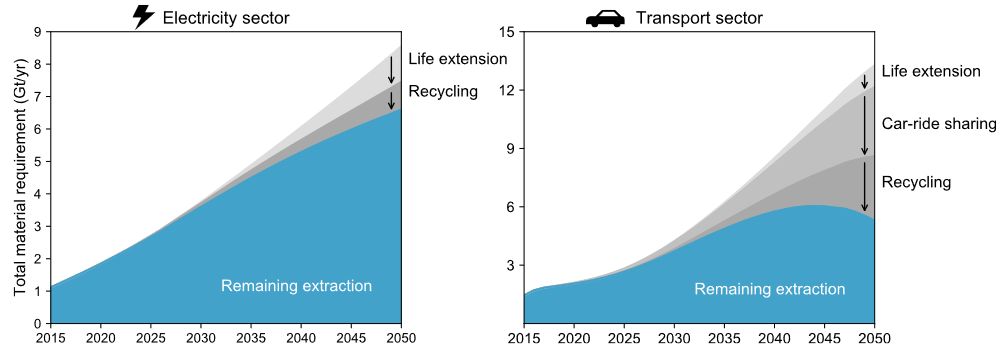
\includegraphics[width=0.7\textwidth]{Images/supply_chain/recycling_scenario.png}
    \caption{Effets sur la quantité de matériaux requis selon plusieurs tendances dans le recyclage, la durée de vie et l'utilisation d'après (\cite{watari_sustainable_2021})}
    \label{fig:recycle}
\end{figure}


